\section{Methodology}
\label{sec:-method}

\subsection{Feature engineering}
The first step in any machine learning problem is to take a look at the 
data, and see what we've gotten ourselves into.  If we start by looking 
at the continuous variables, we observe a number of interesting 
correlations.  

Aspect appears to be somewhat of an outlier in its shape, 
which makes sense when one considers the variable is given in terms of 
degrees: we should be working in modulo 360.  There are a number of 
transformations that could solve this issue: we choose to simply split 
aspect into two different features scaled to 180\degree.

We know that Elevation is measured in meters, as are the 5 other 
``distance to nearest item of interest'' features.  It seems like we 
should be able to do something with that.  In our case, we add the 
differences between Elevation and the Hydrology Distance features.  We 
also integrate the horizontal and vertical distance features, for a 
Euclidian distance measurement. We notice there are some forest cells 
that appear to be nearly underwater, according to the Vertical Distance 
To Hydrology feature.  We introduce a new boolean feature to denote 
that possibility.  

While the graph of wilderness areas appears initially promising (look 
at all of those solid blocks of color!), we note that this is an 
artifact of the graphing process: there are only a few wilderness area 
types, and they seem to be spread pretty evenly among a the cover types.

The soil type graph shows us a preview of one of our more interesting 
discoveries, which we cover more thoroughly in the next subsection. For 
now, we simply observe that some cover types are more distinct from the 
group than others, when we consider solely the soil types.

\subsection{final model}
As we add new features and massage existing features into new shapes, 
we iteratively apply our classifier scheme to the feature vector to 
test the efficacy of those features.  This, however, is not an exact 
science.  A change that increases accuracy over some decisions could 
very well lead to a loss of accuracy over other decisions.  In order to 
more fully examine the consequences of our actions, we make use of a 
graphical tool called a confusion matrix\cite{stehman1997selecting}. A 
confusion matrix, or, error matrix, is a tool suited for specifying 
exactly what kind of missclassifications lead to a loss of accuracy.  
In our case, as we see in Figure \ref{fig:confusion}, our model does a 
pretty good job until we start trying to differentiate between the 
Spruce/Fir type and the Lodgepole Pine type (and, to a lesser extent, 
between Lodgepol Pine and Douglas-fir).  

Adding a mechanism to our ensemble to correct for this error results in 
a modest accuracy increase for our validation set, but a significantly 
greater accuracy gain for the Kaggle competition itself.  If we count 
up the estimated classificaitons, we observe that our classifiers 
predict more 1s and 2s than any other cover type, by nearly an order of 
magnitude.  This suggests that the unexpected gain in accuracy is due 
to a heavier preponderance of Spruce/Fir and Lodgepole Pine trees in 
the testing region.
\begin{figure}
  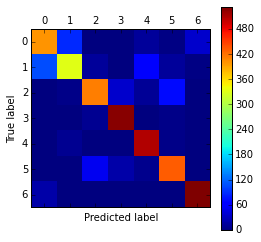
\includegraphics[width=.8\linewidth]{confusion}
 \caption{Confusion Matrix}
 \label{fig:confusion}
\end{figure}
Informed by these features, we then tested a number of classifiers with 
default settings.  Some of these classifiers performed very poorly, 
such as the Naive Bayes algorithm.  We selected several of the best 
performing algorithms, and collected them into a voting body.  
We generated a Support Vector Machine, a Gradient Boosting Machine, and 
a Random Forest classifier on the training data.  We use the weights 
from the Random Forest only to optimize the performance of a k-Nearest 
Neighbor classifier.  That done, we discard the first Random Forest 
weight vector, and train a new Random Forest classifier on a subset of 
training data composed only of cover types 1 and 2.

The GBM, SVM, k-NN classifier, thus assembled, use majority voting to 
determine which classification is selected for a given collection of 
features.  If such a vote results in a classification of cover type 1 
or 2, we fall back to our more select 1/2 Random Forest classifier.

%%% Local Variables: 
%%% mode: latex
%%% TeX-master: "main"
%%% End: 
